\chapter{Diseño e Implementación}


\section{Modelado de la base de datos}
En un primer diagrama para la base de datos se exponen las entidades y sus realciones. Atendiendo a los requisitos de la aplicación se plantea un diseño sencillo y directo en cuanto a las entidades y relaciones. En un primer esquema \textbf{entidad-relación} encontramos:



\begin{figure}[!ht]
  \begin{center}
    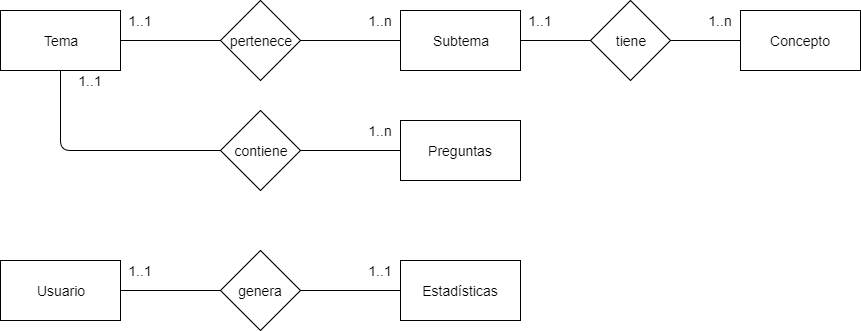
\includegraphics[width=1\textwidth]{../images/entidad_relacion.png}
    \caption{Entidad relación}
    \label{fig:entidad_relacion}
  \end{center}
\end{figure}


\bigskip
Analizando el diagrama vemos que las únicas relaciones que existen son de cardinalidad 1:N y 1:1.
Ambas las podemos simplificar eliminando la relación y añadiendo la clave primaria de la entidad con cardinalidad 1 en los campos de la entidad con cardinalidad N. Quedan así resumidas las tablas de la base de datos a únicamente las entidades:

\begin{figure}[!ht]
  \begin{center}
    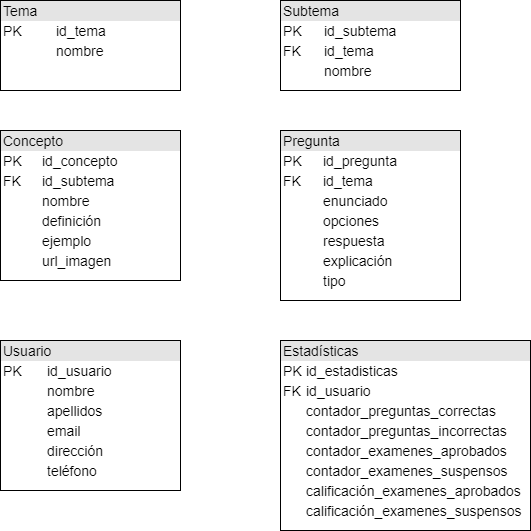
\includegraphics[width=1\textwidth]{../images/entidad_relacion_simplificado.png}
    \caption{Tablas del modelo entidad relación}
    \label{fig:entidad_relacion_simplificado}
  \end{center}
\end{figure}


\newpage

\section{Diseño de las interfaces}

A menudo y varias veces al día nos encontramos con cientos de interfaces\cite{user_exp2} con las que interactuamos, muchas de estas están tan asimiladas que ni las apreciamos. Las interfaces no son un objetivo para el usuario, si no que son el medio para llegar al él, siendo estas que no apreciamos las mejores interfaces. Una interfaz\cite{user_exp} no debe entorpecer el camino del usuario hasta su objetivo, debe ser sencilla, rápida de asimilar y directa.

\bigskip
Aquí mostramos algunos bocetos sencillos y su consiguiente implementación como interfaz de usuario en la aplicación:

\newpage

\subsection{Bocetos}

\begin{figure}[!ht]
  \begin{center}
    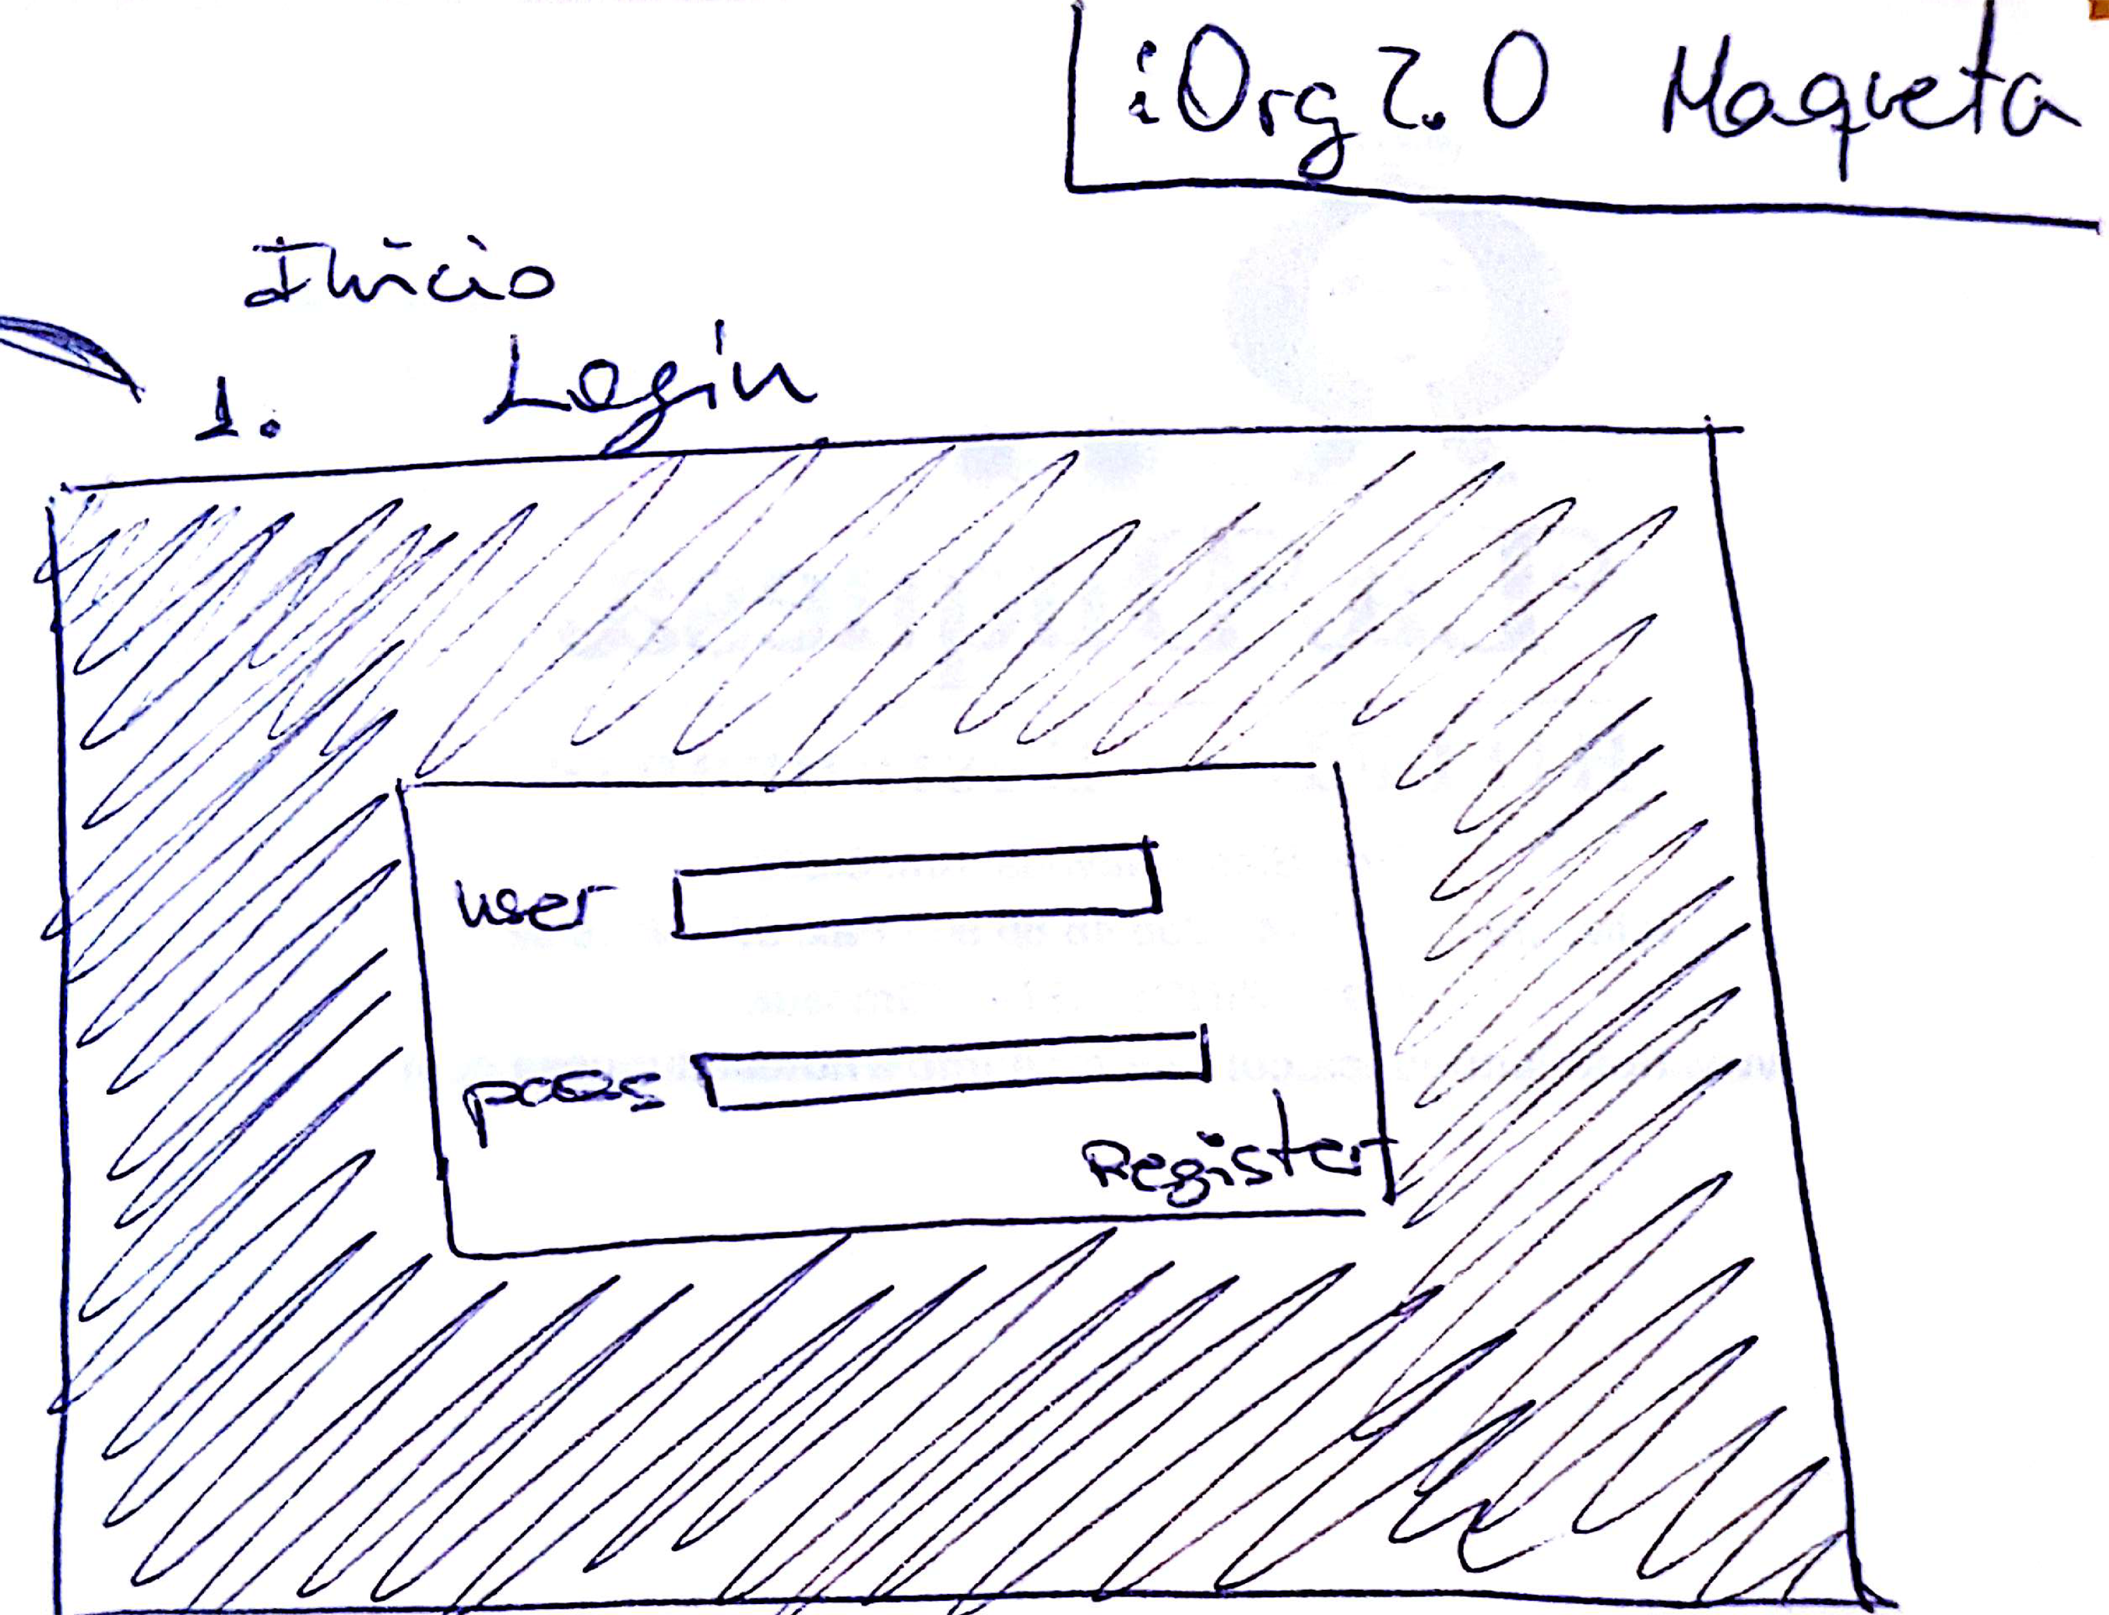
\includegraphics[width=1\textwidth]{../images/boceto_login.png}
    \caption{Boceto interfaz inicio de sesión.}
    \label{fig:boceto_login}
  \end{center}
\end{figure}


\begin{figure}[!ht]
  \begin{center}
    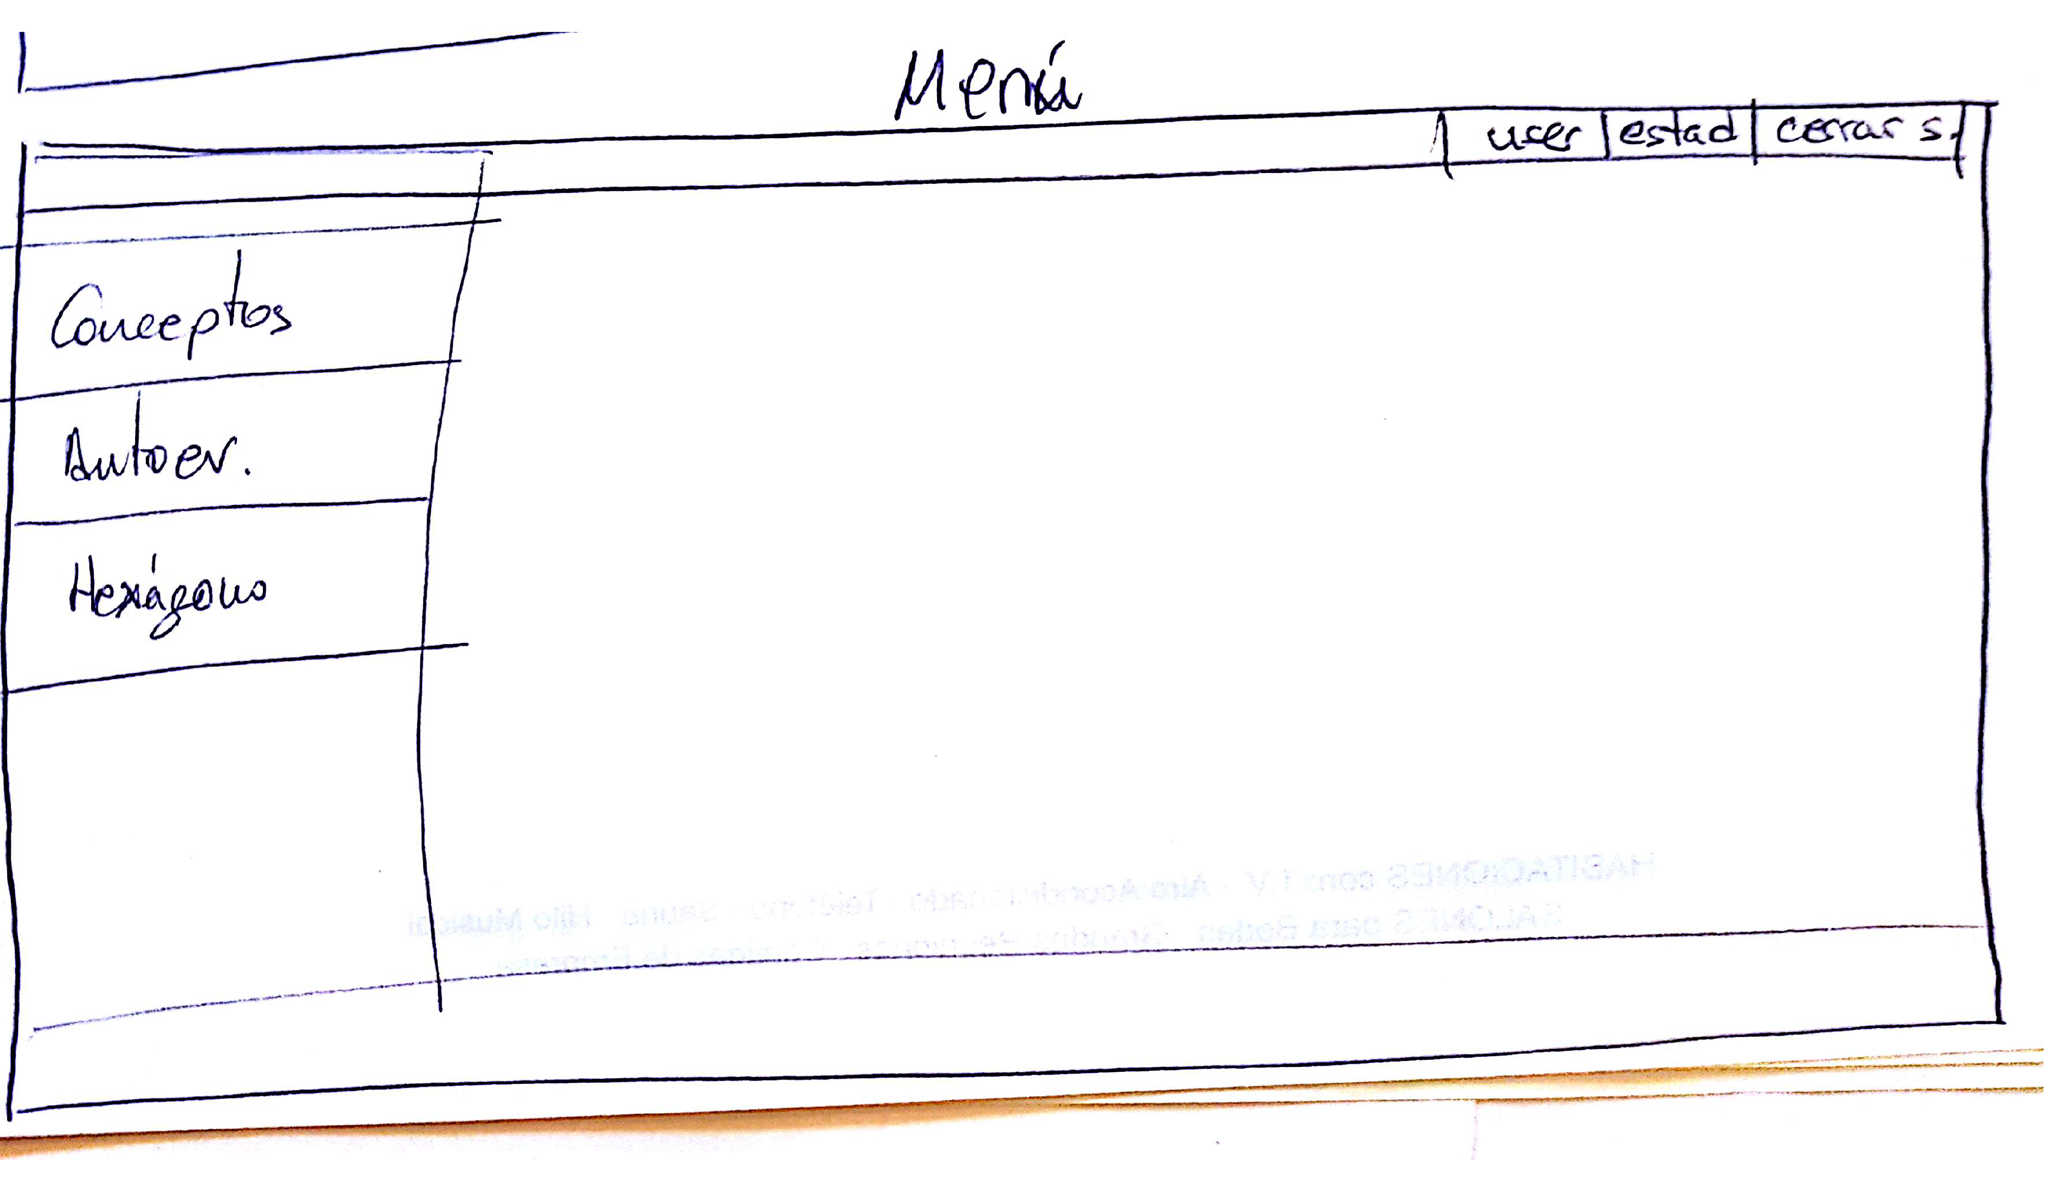
\includegraphics[width=1\textwidth]{../images/boceto_menu_lat.png}
    \caption{Boceto interfaz menú lateral.}
    \label{fig:boceto_menu_lat}
  \end{center}
\end{figure}



\begin{figure}[!ht]
  \begin{center}
    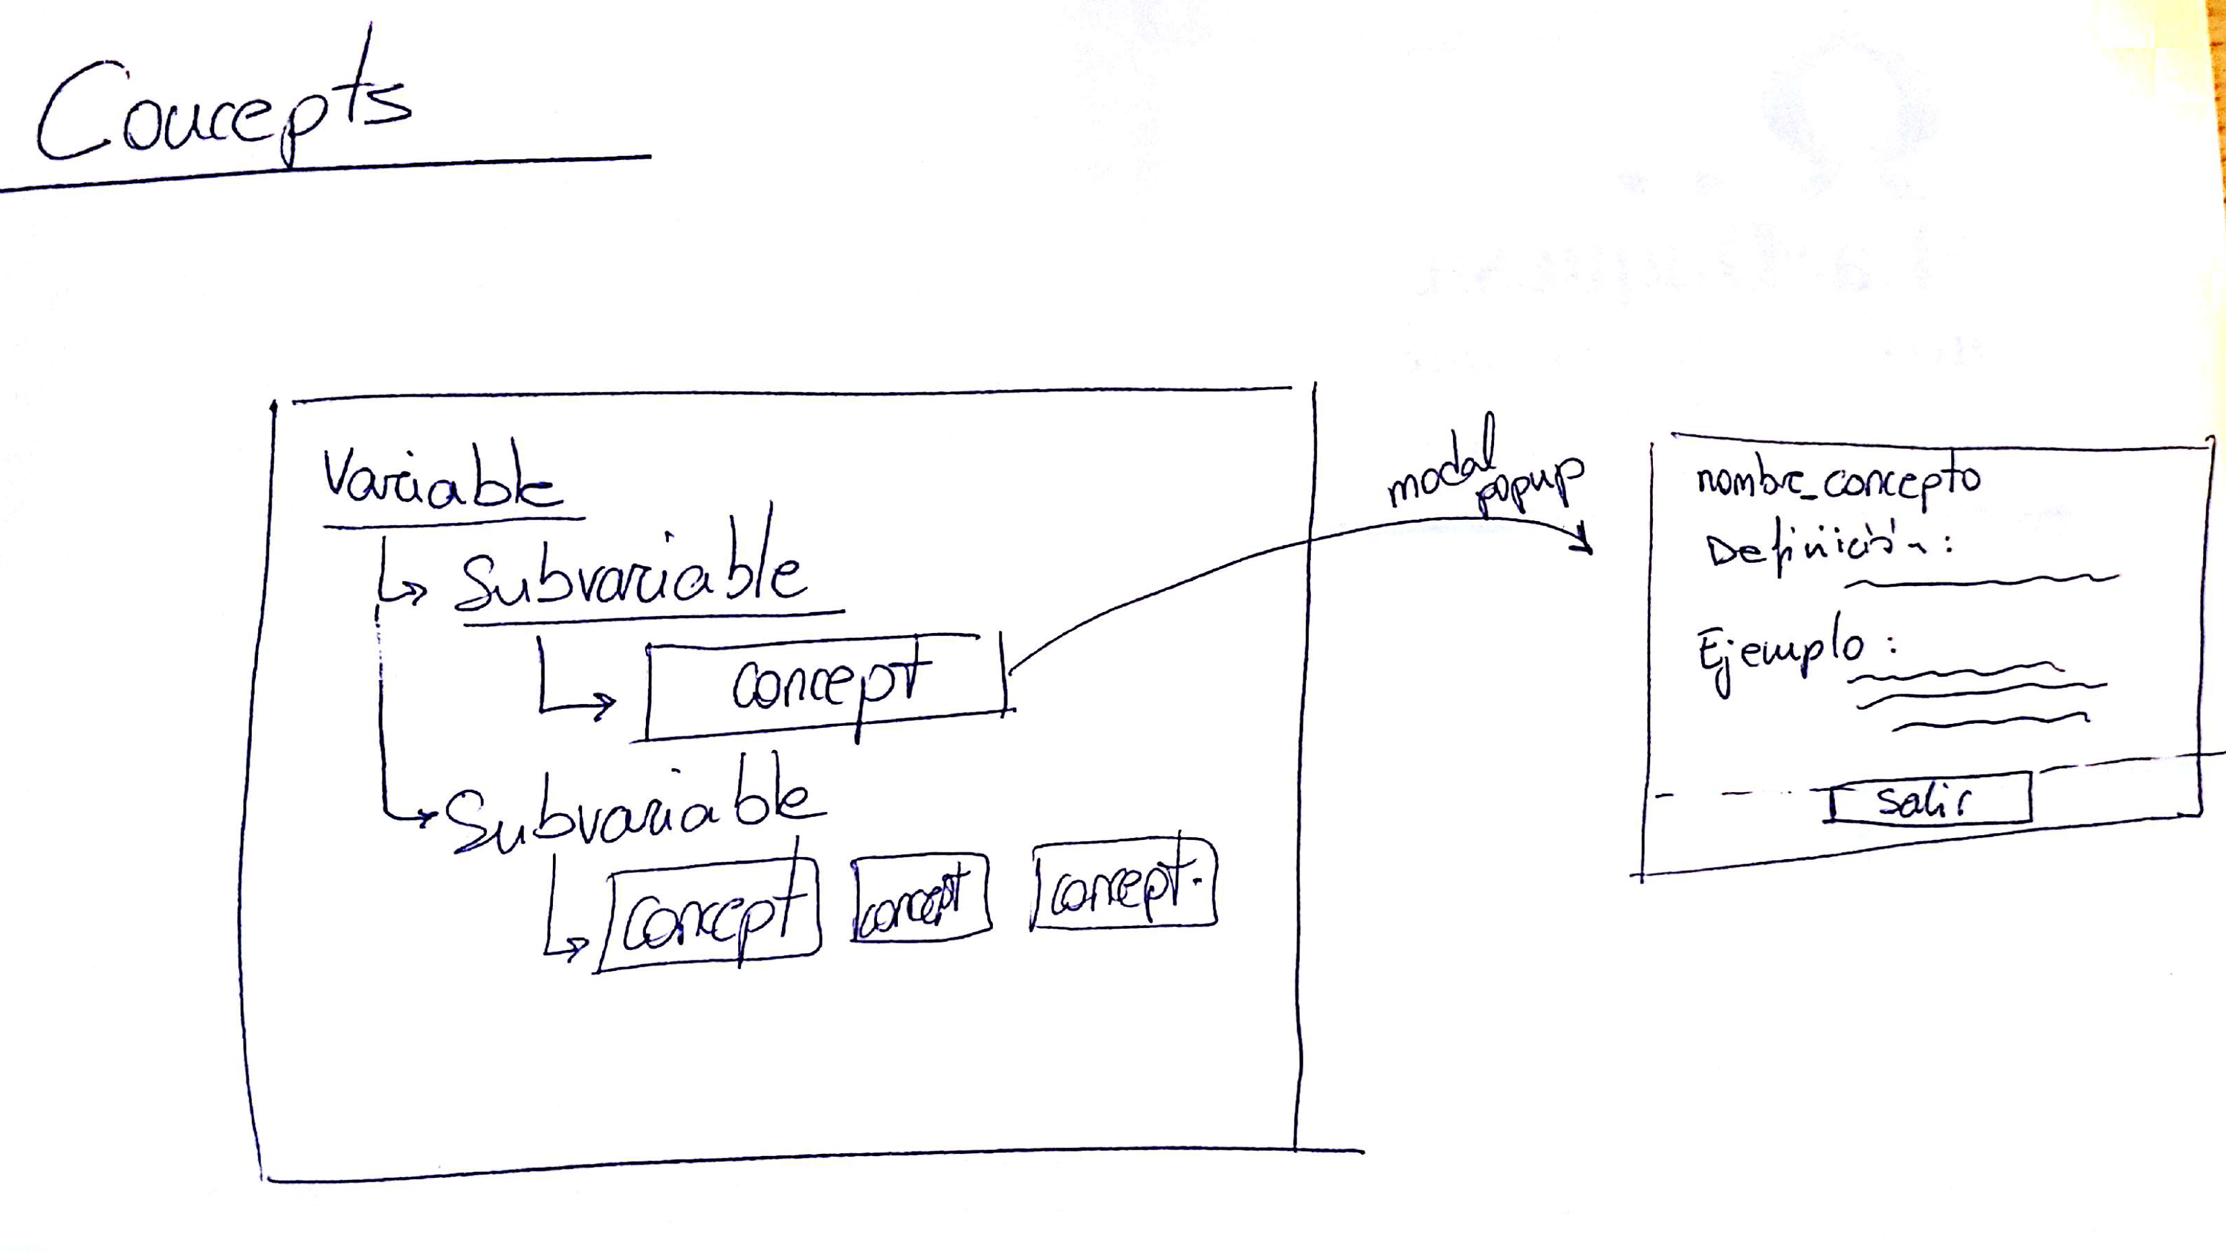
\includegraphics[width=1\textwidth]{../images/boceto_conceptos.png}
    \caption{Boceto interfaz conceptos.}
    \label{fig:boceto_conceptos}
  \end{center}
\end{figure}


\newpage

\subsection{Interfaz}

\begin{figure}[!ht]
  \begin{center}
    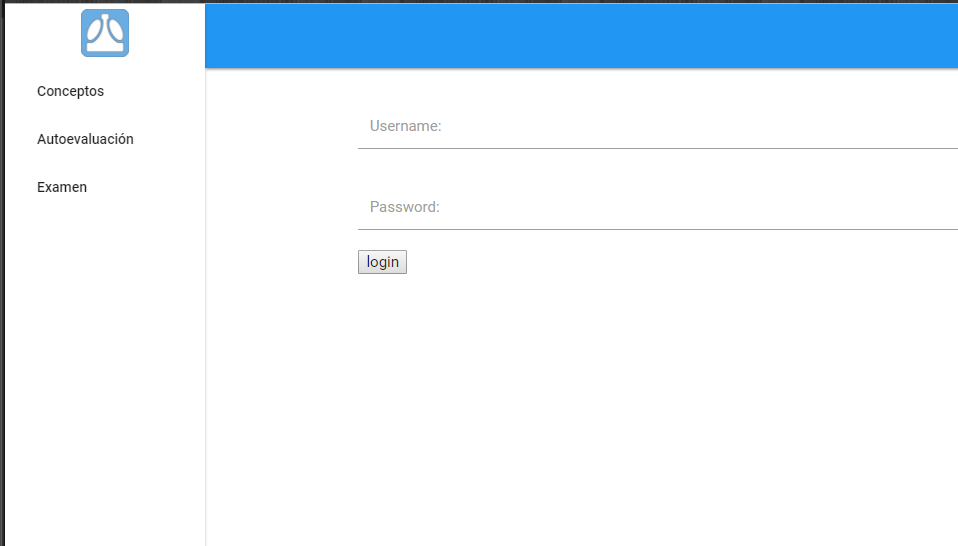
\includegraphics[width=1\textwidth]{../images/interfaz_login.png}
    \caption{Interfaz de usuario inicio de sesión.}
    \label{fig:interfaz_login}
  \end{center}
\end{figure}


\begin{figure}[!ht]
  \begin{center}
    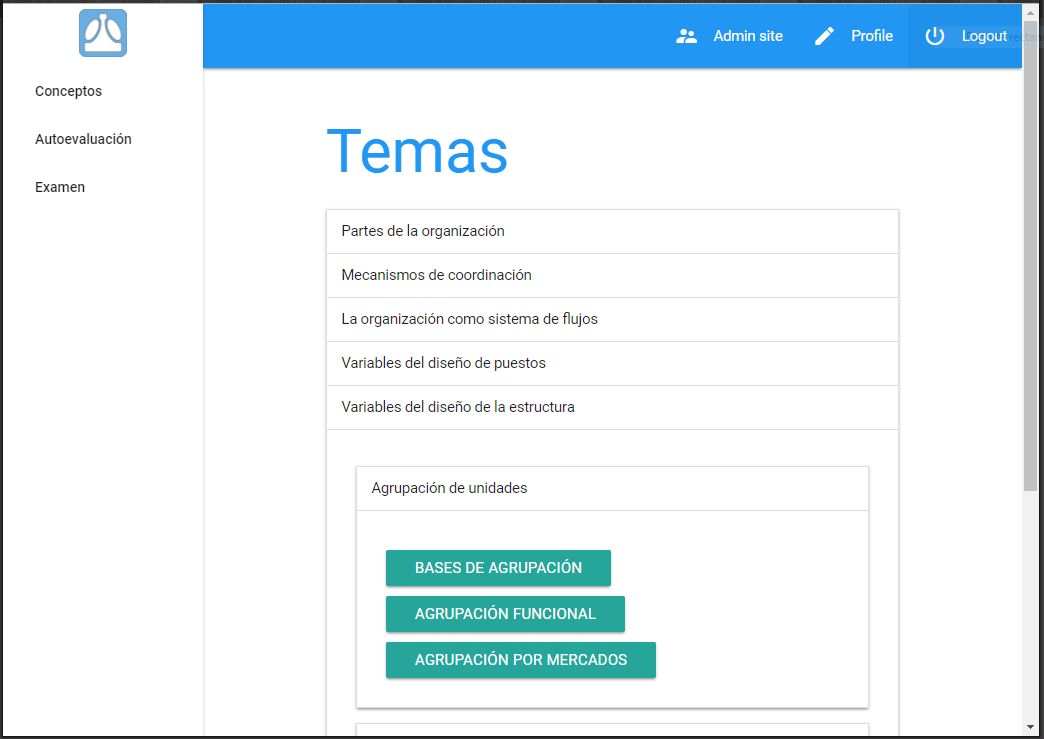
\includegraphics[width=1\textwidth]{../images/interfaz_conceptos1.png}
    \caption{Interfaz de usuario conceptos 1/2.}
    \label{fig:interfaz_conceptos1}
  \end{center}
\end{figure}



\begin{figure}[!ht]
  \begin{center}
    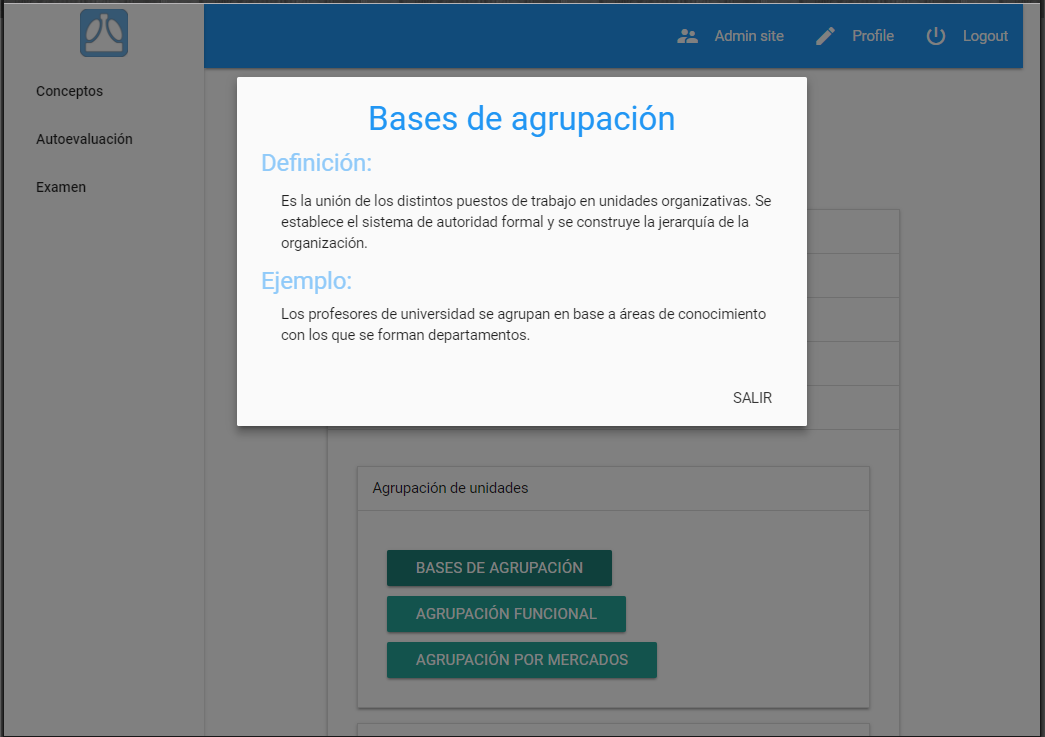
\includegraphics[width=1\textwidth]{../images/interfaz_conceptos2.png}
    \caption{Interfaz de usuario conceptos 2/2.}
    \label{fig:interfaz_conceptos2}
  \end{center}
\end{figure}


\begin{figure}[!ht]
  \begin{center}
    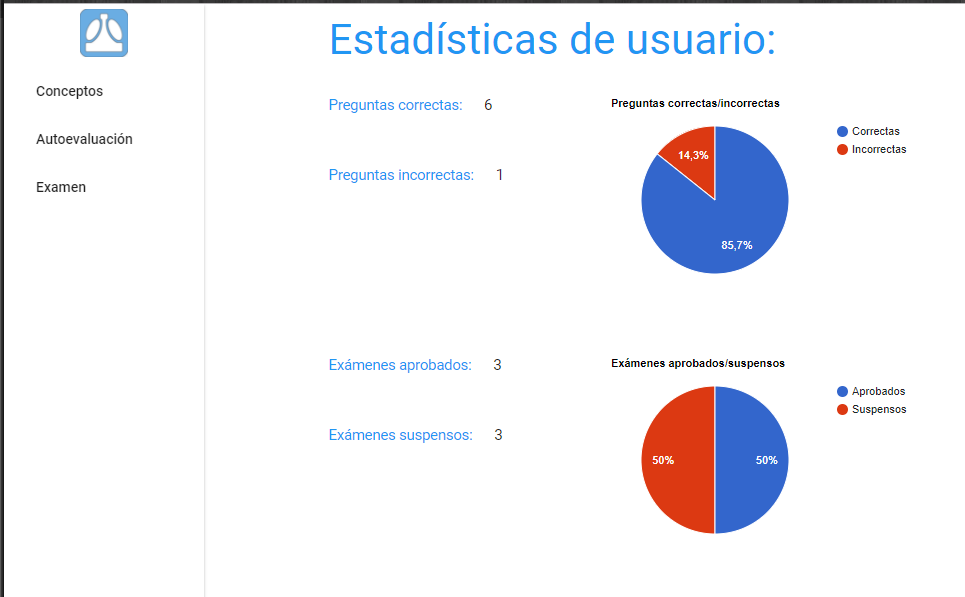
\includegraphics[width=1\textwidth]{../images/interfaz_estadisticas.png}
    \caption{Interfaz de usuario estadísticas de usuario.}
    \label{fig:interfaz_estadisticas}
  \end{center}
\end{figure}



\newpage

\section{Implementación}

